\section{Linear complementary problem}
\subsection{Overview}
A linear complementary problem (LCP) is an optimization problem in which goal is to solve a system of linear equations subject to a complementary condition. In other words, given the matrix $\mathbf{A}\in\mathbb{R}^{d \times d}$ and vector $\mathbf{r}\in\mathbb{R}^{d}$, we want to find the vectors $\mathbf{v}\in\mathbb{R}^{d}$ and $\mathbf{w}\in\mathbb{R}^{d}$ such as
\begin{align*}
  \mathbf{A}\mathbf{v} - \mathbf{w} = \mathbf{b}
\end{align*}
subject to the complementary conditions 
\begin{align*}
  v_i &\ge 0 \qquad \text{for $i = 1,\dots,d$} \\
  w_i &\ge 0 \qquad \text{for $i = 1,\dots,d$} \\
  \mathbf{v}^{T}\mathbf{w} &= 0
\end{align*}
Note that the complementary conditions require that either $v_i=0$ or $w_i=0$ for each component. As you will see later, the pricing problem for American options can be reformulated as a linear complementary problem. But first, we need to reconsider the results obtained from applying the Black-Scholes to pricing problem in section \ref{sec:blackscholes}. Recall that the value curve of American options $V(S,t)$ is bounded from below by the payoff function 
\begin{align*}
  V(S, t) - H(S, t) \ge 0 \qquad \text{for all $(S,t)$}
\end{align*}
Moreover, the value function can be divided in two complementary regions: the exercise region \eqref{eq:blackscholes:preliminaries:exercise_region} where  
\begin{align}
  \label{eq:lcp:overview:value_in_continuation_region}
  &V(S, t) - H(S, t) > 0 \qquad \text{for $(S,t) \in \mathcal{C}$} \\ 
\end{align}
and continuation region \eqref{eq:blackscholes:preliminaries:continuation_region} where 
\begin{align}
  \label{eq:lcp:overview:value_in_exercise_region}
  &V(S, t) - H(S, t) = 0 \qquad \text{for $(S,t) \in \mathcal{S}$}
\end{align}
and the value function $V(S,t)$ is the solution to the Black-Scholes PDE  within the continuation region
\begin{align*}
    \frac{\partial{V}}{\partial{t}} + \mathcal{L}_{\text{BS}}(V) = 0 \qquad \text{for $(S,t) \in \mathcal{C}$}
\end{align*}
where $\mathcal{L}_{\text{BS}}(V)$ is the linear parabolic operator \eqref{eq:blackscholes:preliminaries:linear_parabolic_operator} applied to the function $V(S,t)$. Finally, by plugin $V(S,t)=H(S,t)$ into the Black-Scholes PDE, we obtain the bound for PDE in the exercise region
\begin{align}
    \label{eq:lcp:overview:blackscholes_in_exercise_region}
    \frac{\partial{V}}{\partial{t}} + \mathcal{L}_{\text{BS}} < 0 \qquad \text{for $(S,t) \in \mathcal{S}$}
\end{align}
By grouping \eqref{eq:lcp:overview:value_in_continuation_region}, \eqref{eq:lcp:overview:value_in_exercise_region}, \eqref{eq:lcp:overview:blackscholes_in_exercise_region}, we reformulate the problem of pricing American options as system of variational inequalities
\begin{align}
  \begin{cases}
    \big[\frac{\partial V}{\partial \tau} - \mathcal{L}_{\text{BS}}(V)\big] \cdot [V(S,T-\tau) - H(S,T-\tau)] = 0 & \text{for all $(S,t)$} \\
    V(S, T-\tau) - H(S, T-\tau) \ge 0 & \text{for $(S, t) \ $}\\
    \frac{\partial V}{\partial \tau} - \mathcal{L}_{\text{BS}}(V) \ge 0 &  \text{for all $(S, t)$}\\
    V(S, T) = H(S, T) \\  
  \end{cases}
  \label{eq:lcp:overview:variational_inequalities}
\end{align}
The benefit of the variational inequalities is that there is no explicit dependence on the optimal exercise boundary defined in \eqref{eq:blackscholes:preliminaries:optimal_exercise_boundary}. Also, note that we rewrote the Black-Scholes PDE forward in time by introducing the transformation $\tau = T - t$ deliberately so that the variational inequalities' formulation looks similar in structure to LCP problem. But before elaborating more about the relationship between the variational inequalities and LCP problems, we introduce the transformations
\begin{align}
\label{eq:lcp:overview:heat_diffusion_domain_transformation}
S = Ke^x, \quad t = T - \dfrac{2\tau}{\sigma^2},\quad h(x,\tau) := e^{(\alpha x + \beta \tau)}\dfrac{H(S,t)}{K}, \quad v(x, \tau) := V(S, t) =: Ke^{-(\alpha x + \beta \tau)}y(x, \tau)
\end{align}
where
\begin{align}
  \label{eq:lcp:overview:heat_diffusion_domain_transformation_2}
  q &:= \dfrac{2r}{\sigma^2}, \quad q_{\delta} := \dfrac{2(r-\delta)}{\sigma^2}, \quad \alpha := \dfrac{1}{2}(q_{\delta} - 1) \quad \beta := \dfrac{1}{4}(q_{\delta} - 1)^2 + q 
\end{align}
so that the Black-Scholes PDE \eqref{eq:chapter2:european_option_pde_with_dividens} to transform to the heat diffusion equation
\begin{align}
  \label{eq:lcp:overview:heat_diffusion_equation_PDE}
  \dfrac{\partial{y}}{\partial{\tau}} - \dfrac{\partial^2{y}}{\partial{x^2}} = 0
\end{align}
with boundary conditions, its solution $y(x,\tau)$ lies within the continuous region 
\begin{align}
  \label{eq:lcp:overview:heat_diffusion_equation_solution_region}
  \mathcal{F}: \mathbb{R} \times [0, \sigma^2T/2]
\end{align}
Although we might solve \eqref{eq:lcp:overview:variational_inequalities} without transforming the problem, Dewynne et al. \cite{dewynne_howison_rupf_wilmott_1993} and Seydel \cite{seydel_2009} suggest that transformation to the heat diffusion equation \eqref{eq:lcp:overview:heat_diffusion_equation_PDE} introduces desirable numerical properties when applying finite difference schemes. Hence, under given transformation, the system of variational inequalities \eqref{eq:lcp:overview:variational_inequalities} becomes
\begin{align}
  \begin{cases}
    \bigg[\dfrac{\partial{y}}{\partial{\tau}} - \dfrac{\partial^2{y}}{\partial{x^2}}\bigg] \cdot [y(x, \tau) - h(x, \tau)] = 0 & \text{for all $(x,\tau)$} \\
    y(x, \tau) - h(x, \tau) \ge 0 & \text{for all $(x, \tau)$}\\
    \dfrac{\partial{y}}{\partial{\tau}} - \dfrac{\partial^2{y}}{\partial{x^2}} \ge 0 &  \text{for all $(x, \tau)$}\\
    y(x, 0) = h(x, 0) \\  
  \end{cases}
  \label{eq:lcp:overview:variational_inequalities_heat_equation}
\end{align}
Now that we have formulated the linear complementary problem in terms of the heat equation, we proceed to apply the finite difference scheme framework presented in section \ref{sec:finitedifferencesschemes}. Specifically, we want to approximate $y(x, \tau)$ at each of the nodes within the grid 
\begin{align}
  \mathcal{G} := \{(x_i, \tau_n): (i, n) \in \{0, \dots, M+1\} \times \{0, \dots, N+1\}\}
\end{align}
where 
\begin{align}
  \label{eq:lcp:overview:grid_2}
  x_i &:= x_{\text{min}} + i\Delta{x} &  \qquad \text{for $i = 0,\dots, M+1$} \\
  \tau_n &:= t_{\text{min}} + i{\Delta{\tau}} & \qquad \text{for $i = 0,\dots, N+1$} \\
  \Delta{x} &:= \dfrac{x_{\text{max}} - x_{\text{min}}}{M+1} \\ 
  \Delta{t} &:= \dfrac{t_{\text{max}} - t_{\text{min}}}{N+1}
\end{align}

where $x_{\text{min}}$ is set to a sufficiently small value, $x_{\text{max}}$ to a sufficiently large value, $\tau_{\text{min}}$ to 0 and $\tau_{\text{max}}$ to $\dfrac{\sigma^2}{2}T$

We dedicate the Crank-Nicholson scheme. Moreover, the Crank-Nicholson approximation is given by 
\begin{equation}
  \dfrac{y^{n+1}_{i} - y^{n}_{i}}{\Delta \tau} = \dfrac{1}{2}\bigg(\dfrac{y^{n}_{i-1} - 2y^{n}_{i} + y^{n}_{i+1}}{(\Delta x)^2} + \dfrac{y^{n+1}_{i-1} - 2y^{n+1}_{i} + y^{n+1}_{i+1}}{(\Delta x)^2}\bigg)
\end{equation}

\begin{figure}[H]
  \label{fig:lcp:thetamethod:stencil}
  \centering
  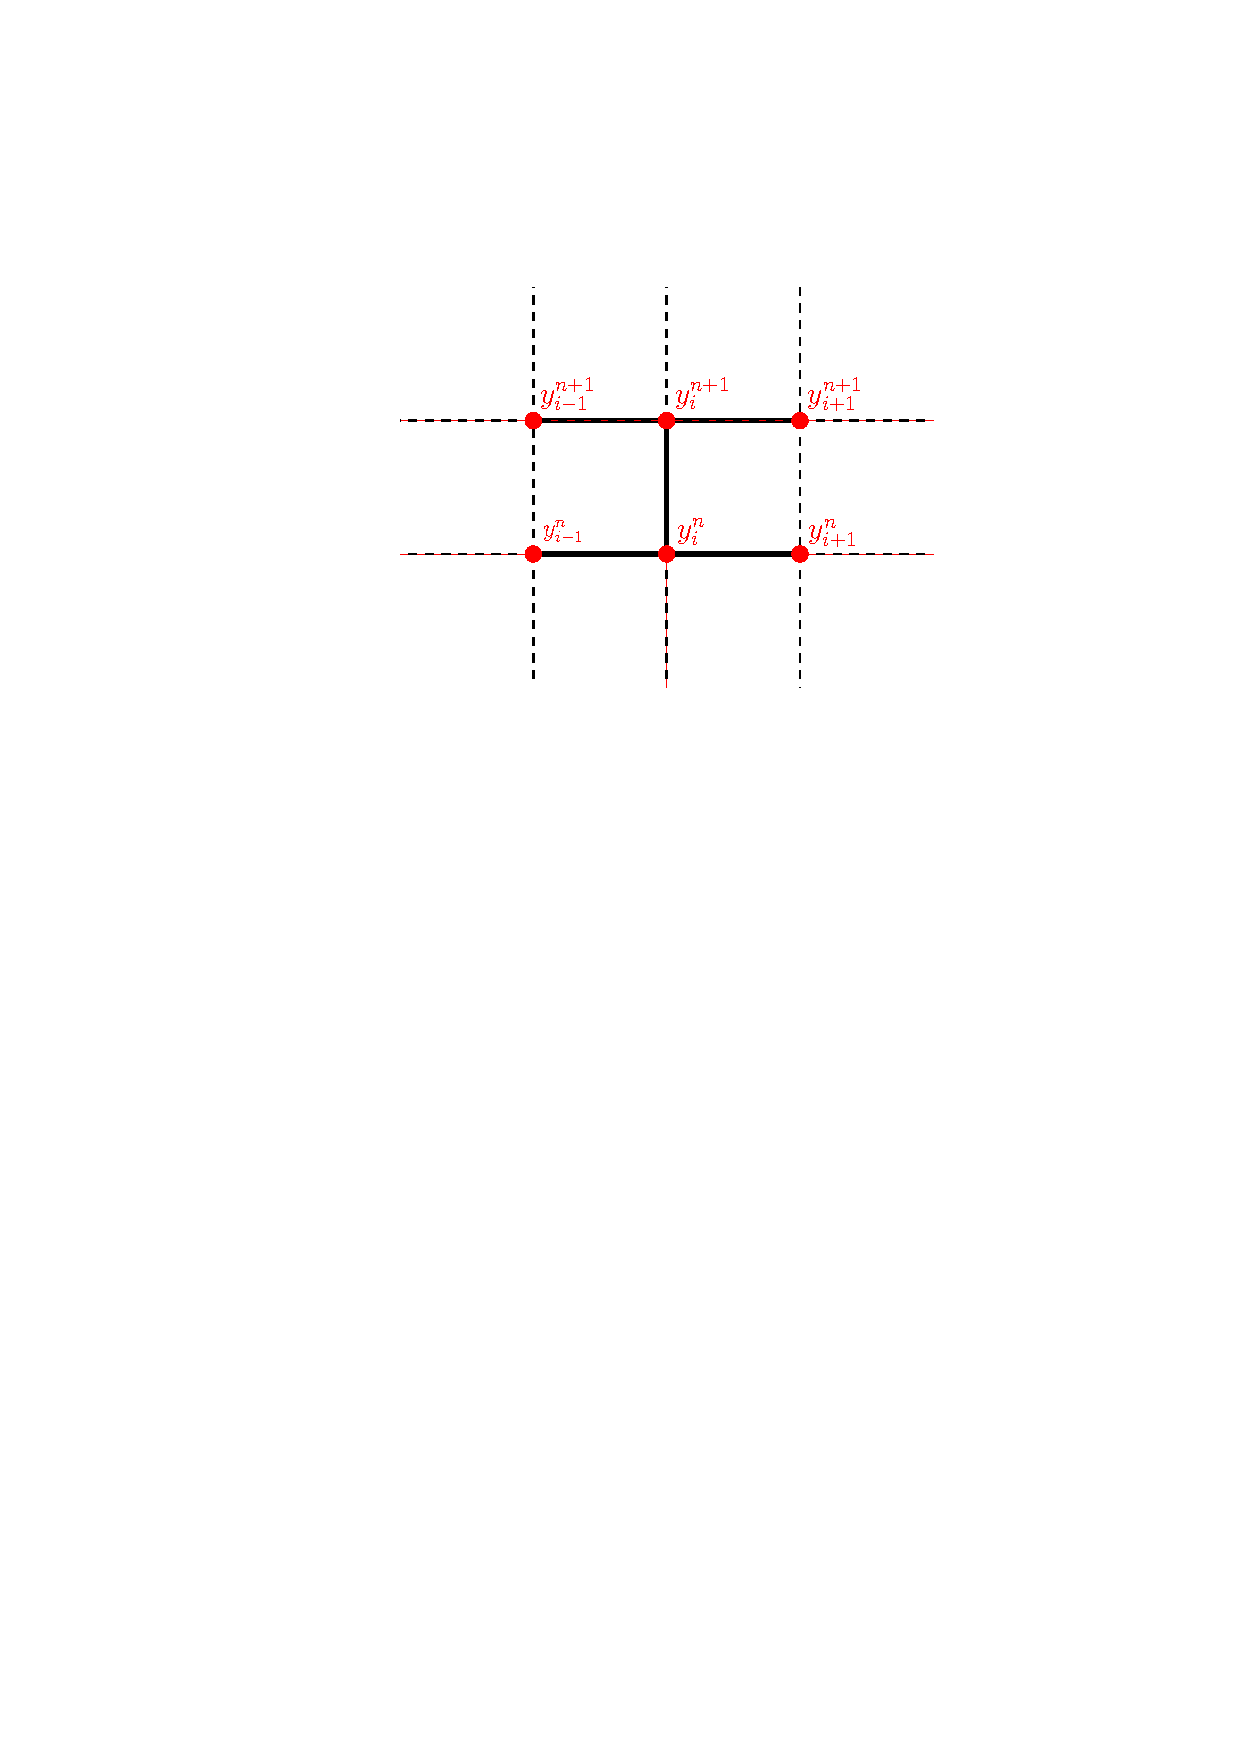
\includegraphics[scale=0.75]{chapters/chapter5/CrankNicholsonStencil.pdf}
  \caption{Stencil diagram for the Crank-Nicholson scheme.}
\end{figure}

\subsection{Theta method}
The theta method is a combination of the explicit and implicit method controlled by parameter $\theta\in[0,1]$
\begin{equation}
  \label{eq:lcp:thetamethod:finitedifference_approximation}
  \dfrac{y^{n+1}_{i} - y^{n}_{i}}{\Delta \tau} = (1-\theta)\dfrac{y^{n}_{i-1} - 2y^{n}_{i} + y^{n}_{i+1}}{(\Delta x)^2} +  \theta\dfrac{y^{n+1}_{i-1} - 2y^{n+1}_{i} + y^{n+1}_{i+1}}{(\Delta x)^2}
\end{equation}
for $i = 1,\dots,M$, and $n = 0,\dots,N$. The PDE approximation is fully explicit for $\theta = 0$, fully implicit for $\theta = 1$, and Crank-Nicholson for $\theta=1/2$. Introducing $\lambda = \Delta{t} / \Delta{x}^2$, and rearranging \eqref{eq:lcp:thetamethod:finitedifference_approximation}, we have
\begin{equation}
  \label{eq:lcp:thetamethod:finitedifference_approximation_2}
  y^{n+1}_{i} - \lambda\theta(y^{n+1}_{i-1} - 2y^{n+1}_{i} + y^{n+1}_{i+1}) =  y^{n}_{i} + (1-\theta)\lambda(y^{n}_{i-1} - 2y^{n}_{i} + y^{n}_{i+1})
\end{equation}
for $i = 1,\dots,M$, and $n = 0,\dots,N$. Also, let us define $b^n_i$
\begin{equation}
  b^{n}_i := y^{n}_{i} + (1-\theta)\lambda(y^{n}_{i-1} - 2y^{n}_{i} + y^{n}_{i+1})
\end{equation}
for $i = 1,\dots,M$, and $n = 0,\dots,N$. Then, we define the vectors $\mathbf{b}^n\in\mathbb{R}^{M}$, $\mathbf{y}^{n+1}\in\mathbb{R}^{M}$ and $\mathbf{h}^n\in\mathbb{R}^{M}$ ad
\begin{align}
  \mathbf{b}^{n} :=& \begin{bmatrix}
    b^{n}_1, \dots, b^{n}_{M}
  \end{bmatrix}^{T}\\
  \mathbf{y}^{n+1} :=& \begin{bmatrix}
    y^{n+1}_1, \dots, y^{n+1}_{M}
  \end{bmatrix}^{T}\\
  \mathbf{h}^{n+1} :=& \begin{bmatrix}
    h(x_1, \tau_{n+1}), \dots, h(x_M, \tau_{n+1})
  \end{bmatrix}^{T}
\end{align}
and the matrix $\mathbf{A}\in\mathbb{R}^{M \times M}$ as
\begin{align}
  A :=& \begin{bmatrix}
    1+2\theta & -\lambda\theta & & 0 \\ 
   -\lambda\theta & \ddots & \ddots \\
      & \ddots & \ddots & \ddots \\
    0 & & \ddots & \ddots & \\
  \end{bmatrix} 
\end{align}
Hence, we can write the equations in \eqref{eq:lcp:overview:variational_inequalities_heat_equation} as  
\begin{align}
  \begin{cases}
    (\mathbf{A}\mathbf{y}^{n+1} + \mathbf{b}^{n})^{T}(\mathbf{y}^{n+1}- \mathbf{h}^{n+1}) = 0\\
    \mathbf{A}\mathbf{y}^{n+1} + \mathbf{b}^{n} \ge 0\\
    \mathbf{y}^{n+1}- \mathbf{h}^{n+1} \ge 0 \\
    \mathbf{y}^{0} = \mathbf{h}^{0} \\  
  \end{cases}
  \label{eq:lcp:overview:variational_inequalities_heat_equation_2}
\end{align}
which is the LCP formulation. Note that if we define the vectors
\begin{align*}
  \mathbf{v} := \mathbf{y}^{n+1} - \mathbf{h}^{n+1} \\
  \mathbf{w} := \mathbf{A}\mathbf{y}^{n+1} - \mathbf{b}^{n} \\
  \mathbf{r} := \mathbf{b}^n - \mathbf{A}\mathbf{h}^{n+1}
\end{align*}

\begin{align}
    b^{n}_{i} := y^{n}_{i} + (1-\theta)\lambda(y^{n}_{i-1} - 2y^{n}_{i} + y^{n}_{i+1})
\end{align}

\begin{align}
  h^{n}_{i} := h(x_i, \tau_n)
\end{align}

\subsection{PSOR method}

\subsection{Numerical results}